\chapter{Opis projektnog zadatka}

    \section{Cilj i opis zadatka}
    Cilj ovog projekta je razviti programsku podršku za web aplikaciju "Dog Friendly" koja će omogućiti korisnicima da na interaktivnoj karti pronađu prikladne lokacije za druženje sa svojim ljubimcima i time im olakšati kretanje. U svrhu financiranja aplikacije, omogućit ćemo vlasnicima obrta koja su povezana sa psima da postave svoju reklamu na stranicu uz određenu pretplatu.
    
    \section{Problematika zadatka}
    Aplikacija Dog Friendly omogućuje svojim korisnicima kretanje po interaktivnoj karti, ručni unos tržene adrese te, uz dozvolu, lociranje vlastitog uređaja. Korisnici pristupaju aplikaciji preko web stranice gdje se mogu prijaviti kao osnovni korisnik ili vlasnik obrta. Odabirom vrste korisnika im se otvara tražena registracijska forma.
    \newline 
    Za stvaranje računa osnovnog korisnika potrebno je:
        \begin{itemize}
            \item \textbf{ime}
            \item \textbf{prezime}
			\item \textbf{korisničko ime} 
			\item \textbf{e-mail} 
			\item \textbf{lozinku}
			\item \textbf{opis}
		\end{itemize}
    Registriranim korisnicima je osim osnovnih funkcija omogućeno postavljanje novih lokacija, označavanje lokacija prikladnim/neprikladnim za pse, ostavljanje recenzija i komentara na lokacije. 
    \eject
    Za vlasnike obrta je dodatno potrebno unijeti:
    \begin{itemize}
		\item \textbf{ime obrta} 
		\item \textbf{OIB} 
		\item \textbf{e-mail}
		\item \textbf{lozinka}
		\item \textbf{broj telefona}
		\item \textbf{opis}
		\item \textbf{tip obrta}
		\item \textbf{broj kartice}
		\item \textbf{CVV}
		\item \textbf{datum isteka kartice}
	\end{itemize}
	Vlasnici obrta nakon registracije na karti odabiru adrese svojih obrta i postavljaju na njih markere. Prilikom odabira lokacije osnovnom korisniku se prikazuje adresa i javni dio podataka unesen prilikom registracije (ime obrta, kontakt i opis). Na dnu obrasca za registraciju se nalazi "mock" obrazac za unos kartičnih podataka (obavezno za vlasnike obrta).
	\newline
    
    \section{Korisnički zahtjevi}
    \hfill\break
    \textbf{Neregistrirani korisnik} može se kretati po karti i vidjeti sve prikladne i neprikladne lokacije i plaćene lokacije (obrte) koje su mu dodatno istaknute. U polju za pretragu može unijeti specifičnu lokaciju koja će mu se centrirati na karti. Moguće je odabrati kategoriju čiji se markeri onda prikazuju. Klikom na marker moguće je saznati više informacija o lokaciji kao što su njezin naziv, ocjena i tip lokacije. Klikom na marker obrta dodatno je moguće vidjeti naziv, adresu, opis obrta i kontakt. Osim toga, korisnik može omogućiti lociranje vlastitog uređaja. 
     \newline
    Korisnik može poslati zahtjev za registracijom te potom ispuniti tražene podatke. Registracija se potvrđuje preko e-mail potvrde i korisnik dobiva potvrdu o uspješnoj registraciji. Vlasnik obrta uz potvrdu o registraciji dobiva i potvrdu o plaćanju. 
    \newline
    \hfill\break
    \textbf{Osnovnom korisniku} je, osim svih funkcionalnosti neregistriranog korisnika, omogućeno označavanje lokacija kao prikladne i neprikladne. Prilikom označavanja potrebno je unijeti ime lokacije i odabir kategorije iz izbornika. Također za već postojeće lokacije moguće je potvrditi ili negirati postojeću oznaku i dodati recenziju. Korisniku je omogućena promjena korisničkog imena i lozinke. 
    \newline
    \hfill\break
    \textbf{Vlasnik obrta} može pregledavati i odgovati na recenzije svog obrta. Omogućena mu je promjena korisničkog imena i lozinke, promjena naziva, opisa i kategorije obrta te dodavanje jedne ili više adresa na kojima se obrt nalazi. Pretplatom na aplikaciji osigurava da njegove lokacije budu drugačije istaknute od običnih lokacija.
    
    \section{Inovacije koje pruža}
    Aplikacija bi bila prva takva u Hrvatskoj koja ne samo da pruža pronalazak prikladnih lokacija za pse, nego korisnici mogu pronaći i neprikladne lokacije kako bi ih mogli izbjeći. Osim toga, aplikacija nudi i prikaz obrta kao što su: pet shopovi, veterinarske ordinacije, frizerski saloni za pse, itd. To omogućuje našim korisnicima da na jednom mjestu pronađu sve potrebno za njihove ljubimce.
    
    \section{Slični projekti}
    Pronalazak parkova za pse i različitih potrepština je posebno izazovan za nove vlasnike i korisnike koji se po prvi put nađu u novom gradu. Zbog toga na tržištu postoji potreba za ovakvom aplikacijom, ali i slična rješenja
    \newline
    \textbf{DogPack} \newline
    DogPack je mobilna aplikacija koja uključuje detaljnu kartu parkova za pse u brojnim zemljama, pa tako i Hrvatskoj. Nudi mogućnost lokacije traženog parka, prijave za dolazak u odabrani park i popis trenutnih posjetitelja parku.Aplikacija korisnicima omogućuje izradu profila, komunikaciju s drugim korisnicima, objavljivanje slika i videozapisa i slično.  
    \begin{figure}[H]
        \centering
        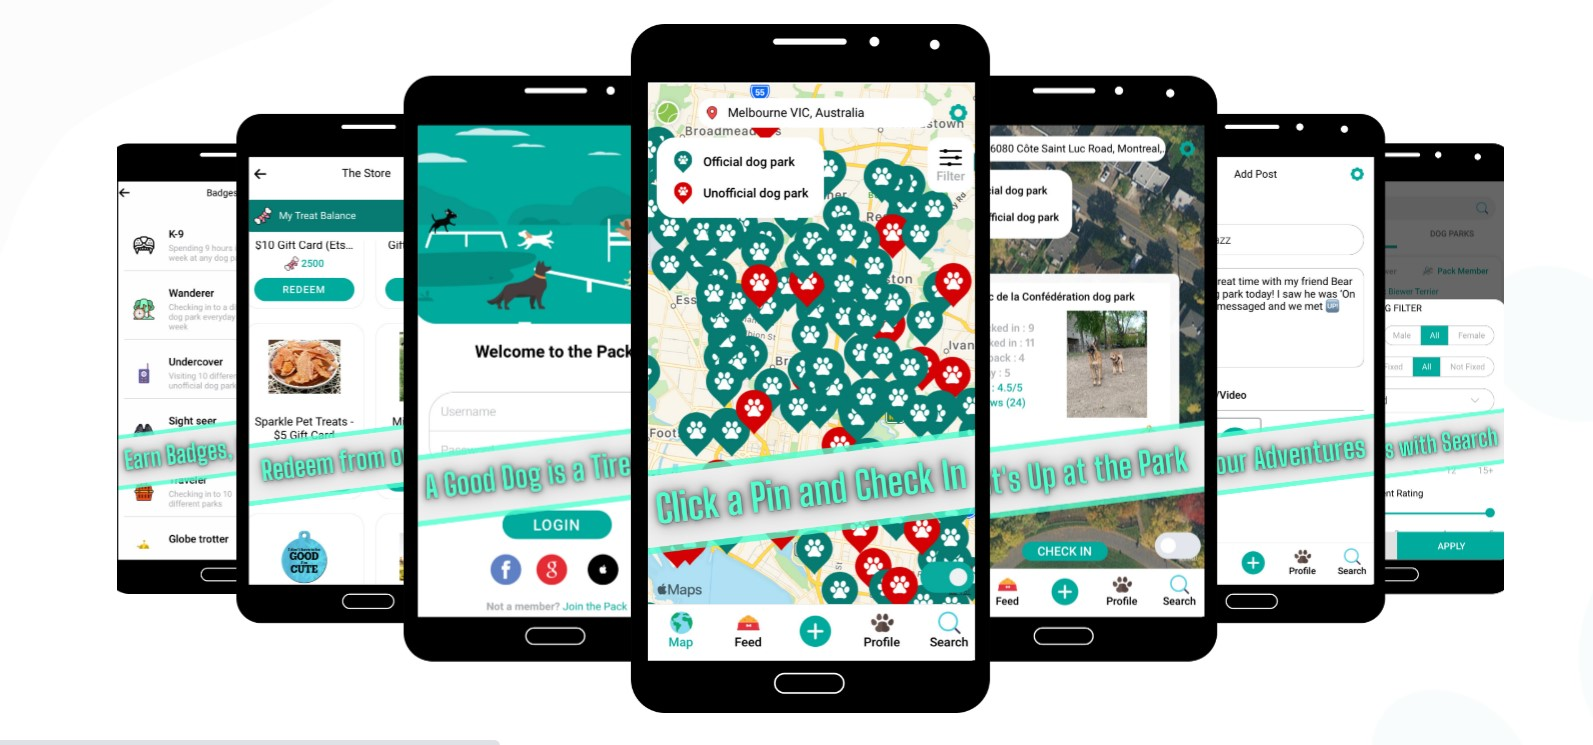
\includegraphics[width=\textwidth]{img/DogPack.jpg}
        \caption{Prikaz mogućnosti koje nudi aplikacija DogPack}
    \end{figure}
    
    
    \textbf{Dog Park Finder} \newline
    Aplikacija tvrtke Nylabone omogućuje korisnicima da unesu svoj poštanski broj i radius pretrage i aplikacija prikazuje na interaktivnoj karti lokacije svih parkova za pse u zadanom radiusu. Aplikacije je ograničena na korisnike iz SAD-a. 
    \begin{figure}[H]
        \centering
        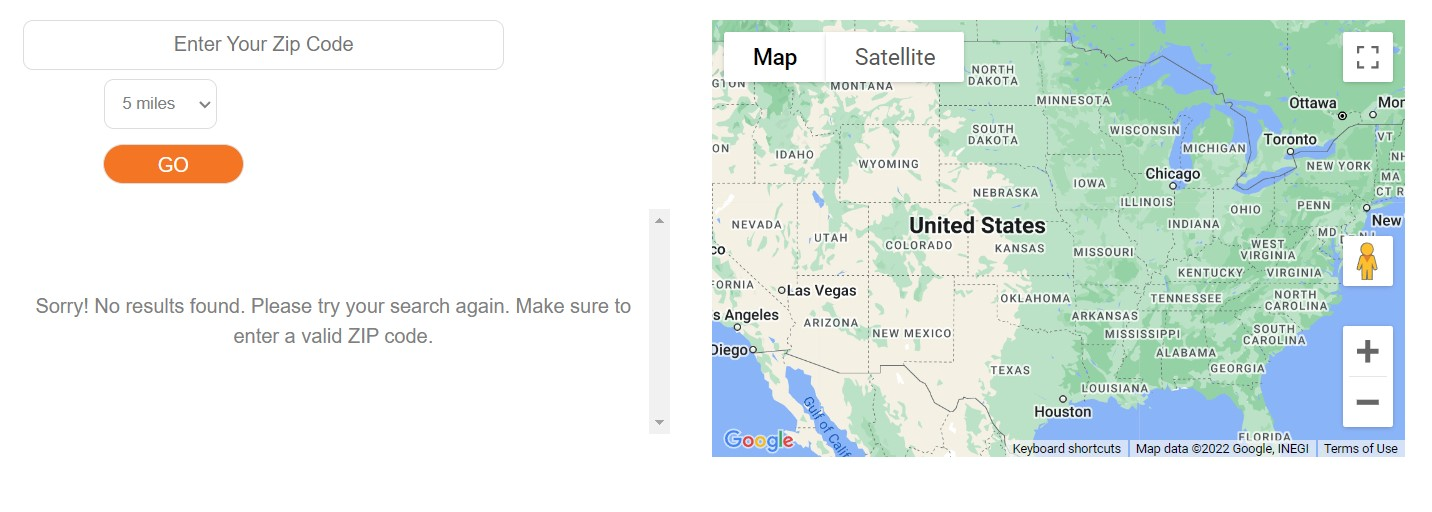
\includegraphics[width=\textwidth]{img/DogParkFinder.jpg}
        \caption{Prikaz karte}
    \end{figure}
    \textbf{Sniffspot} \newline
    Aplikacija omogućuje svojim korisnicima da unajme sigurne i privatne pseće parkove gdje možete sami sa svojim ljubimcem provoditi kvalitetno vrijeme. Aplikacija je ograničena na korisnike iz SAD-a.
    
	
		
		
		